\documentclass[11pt,compress,t,notes=noshow, aspectratio=169, xcolor=table]{beamer}

\usepackage{../../style/lmu-lecture}
% Defines macros and environments
% This file is included in slides and exercises

% Rarely used fontstyle for R packages, used only in 
% - forests/slides-forests-benchmark.tex
% - exercises/single-exercises/methods_l_1.Rnw
% - slides/cart/attic/slides_extra_trees.Rnw
\newcommand{\pkg}[1]{{\fontseries{b}\selectfont #1}}

% Spacing helpers, used often (mostly in exercises for \dlz)
\newcommand{\lz}{\vspace{0.5cm}} % vertical space (used often in slides)
\newcommand{\dlz}{\vspace{1cm}}  % double vertical space (used often in exercises, never in slides)
\newcommand{\oneliner}[1] % Oneliner for important statements, used e.g. in iml, algods
{\begin{block}{}\begin{center}\begin{Large}#1\end{Large}\end{center}\end{block}}

% Don't know if this is used or needed, remove?
% textcolor that works in mathmode
% https://tex.stackexchange.com/a/261480
% Used e.g. in forests/slides-forests-bagging.tex
% [...] \textcolor{blue}{\tfrac{1}{M}\sum^M_{m} [...]
% \makeatletter
% \renewcommand*{\@textcolor}[3]{%
%   \protect\leavevmode
%   \begingroup
%     \color#1{#2}#3%
%   \endgroup
% }
% \makeatother


\title{Interpretable Machine Learning}
% \author{LMU}
%\institute{\href{https://compstat-lmu.github.io/lecture_iml/}{compstat-lmu.github.io/lecture\_iml}}
\date{}

\begin{document}

% Set style/preamble.Rnw as parent.
\newcommand{\vertiii}[1]{{\left\vert\kern-0.25ex\left\vert\kern-0.25ex\left\vert #1 
    \right\vert\kern-0.25ex\right\vert\kern-0.25ex\right\vert}}
% Load all R packages and set up knitr

% This file loads R packages, configures knitr options and sets preamble.Rnw as 
% parent file
% IF YOU MODIFY THIS, PLZ ALSO MODIFY setup.Rmd ACCORDINGLY...

% Defines macros and environments
 \newcommand{\titlefigure}{figure/AEloanApplication.png} 
\newcommand{\learninggoals}{
\item Compare adversarial examples to counterfactual explanations
\item See an example where both coincident}

\lecturechapter{\Large{Adversarial Examples and Counterfactual Explanations}}
\lecture{Interpretable Machine Learning}

% ------------------------------------------------------------------------------

\begin{vbframe}{ADE and Counterfactual Explanations}
It seems as if ADEs and counterfactual explanations (CEs) are defined similarly. Both ADEs and CEs describe inputs close to a given input $\xv$ that gets a different assignment. What are their differences?
\begin{itemize}
    \item Counterfactuals do not have to be misclassified.
%    \item Counterfactuals should be maximally close to $\xv$.
    \item Different notions of distance $\|\cdot\|$ are applied, e.g., $p_{2,\infty}$-norm for ADEs or $p_{0,1}$-norm for CEs.
    \item Informal difference I: ADEs are mostly considered for high-dimensional data, while CEs are mostly considered in the context of low-dimensional data.
    \item Informal difference II: ADEs hide changes while CEs highlight them.
\end{itemize}
\end{vbframe}

\begin{vbframe}{Shared Example \citebutton{Ballet (2019)}{https://arxiv.org/pdf/1911.03274.pdf}}
\begin{itemize}
\item \textbf``If you had two more pets, your loan application would have been granted" is an example of both ADEs and CEs.
\end{itemize}
\begin{figure}[h]
\centering
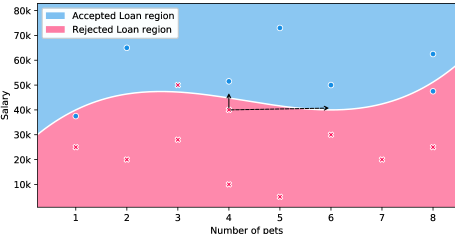
\includegraphics[width=0.6\linewidth]{figure/AEloanApplication.png}\\
   \centering
  {Decision boundary of a classifier deciding loan applications. ADE via ``number of pets''}
  \label{fig:mnist}
\end{figure} 
\end{vbframe}

\endlecture
\end{document}

